\section{Exercises}

These exercises are taken from the course workbook\cite{exerciseBook}. In the following sections you can see how we approached the exercises.

\subsection{Availability}

\subsubsection{Collection and analysis}

\descriptionproblem
Consider the system in Figure~\ref{fig: exercises - collection and analysis system}. Assume that the participating components offer the following availability:
\begin{itemize}
    \item \texttt{DataCollector}: 99\%
    \item \texttt{MessageQueue}: 99.99\%
    \item \texttt{DataAnalyzer}: 99.5\%
\end{itemize}

\begin{figure}[!htp]
    \centering
    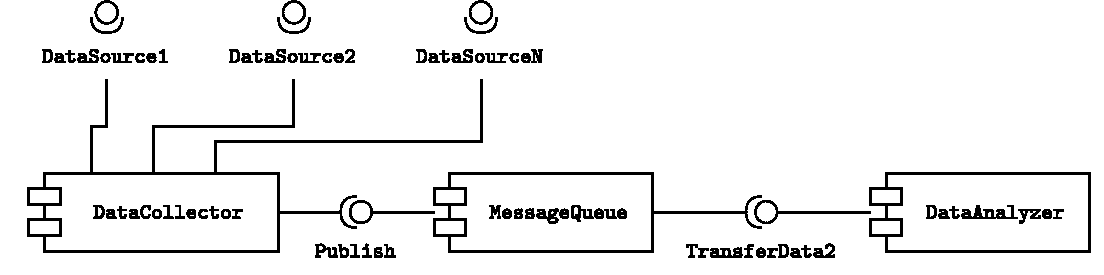
\includegraphics[width=\textwidth]{img/collection-and-analysis-1.pdf}
    \caption{Collection and analysis system.}
    \label{fig: exercises - collection and analysis system}
\end{figure}

\questionproblem
\begin{enumerate}
    \item Provide an estimate of your system's total availability (a rough estimation is acceptable without complete calculations). Assume you want to improve this total availability through replication, which component(s) would you choose to replicate? Explain your reasoning.
    
    \item How would such replication impact the way the system works and is designed?
\end{enumerate}

\solution
\textbf{\underline{Solution 1}.} We can use Equation~\ref{eq: availability in series} on page~\pageref{eq: availability in series} to estimate our system's total availability. Then, we can multiply the availability of each item in the system:
\begin{equation*}
    \begin{array}{rcl}
        \texttt{Availability} &=& \texttt{DataCollector} \times \texttt{MessageQueue} \times \texttt{DataAnalyzer} \\ [.5em]
        %
        &=& \left(99 \div 100\right) \times \left(99.99 \div 100\right) \times \left(99.5 \div 100\right) \\ [.5em]
        %
        &=& 0.99 \times 0.9999 \times 0.995 \\ [.5em]
        %
        &=& 0.984951495 \approx 0.985
    \end{array}
\end{equation*}
Now, we want to improve the system's accessibility. As the exercise suggests, we use the replication technique. Since the component to replicate is the worst, we replicate the \texttt{DataAnalyzer} (99.5\% availability).

So, how can we calculate accessibility? Well, when we replicate a component, we take advantage of the \emph{parallel} concept. Then, we use Equation~\ref{eq: availability in parallel} (page~\pageref{eq: availability in parallel}) on these components. Finally, the availability becomes:
\begin{equation*}
    \begin{array}{rcl}
        \texttt{Improved Avail.} &=& 0.99 \times 0.9999 \times \left[1 - \left(1 - 0.995\right)\times\left(1 - 0.995\right)\right] \\ [.5em]
        %
        &=& 0.989901 \times \left[1 - 0.000025\right] \\ [.5em]
        %
        &=& 0.989901 \times 0.999975 \\ [.5em]
        %
        &=& 0.989876252475 \approx 0.989 \approx 0.99
    \end{array}
\end{equation*}

\highspace
\textbf{\underline{Solution 2}.} We have improved the availability system with replication, but how are two parallel components managed? We can choose between three available tactics (page~\pageref{Replication approaches}): Hot Spare, Warm Spare, and Cold Spare (\emph{Triple Modular Redundancy} cannot be applied because there are only two parallel modules).
\begin{itemize}
    \item \emph{Hot Spare} approach: \texttt{DataCollector1} and \texttt{DataCollector2} are updated at the same time from the \texttt{MessageQueue}. One component leads, and another is always ready to take over.
    
    However, the main problem with this choice is the \emph{data duplication}. Because when the two components receive the same data, both process and return the information at the source \texttt{MessageQueue}. To manage this issue, we can code a system to avoid duplicates on the queue. 
    
    Another issue when two sources answer simultaneously is \emph{concurrency} (a race condition problem). This problem can be solved by implementing mutual exclusion mechanisms.


    \item \emph{Warm} or \emph{Cold Spare}: In the first, \texttt{DataCollector1} leads and periodically updates the \texttt{DataCollector2}. If the primary \texttt{DataCollector} fails, the second \texttt{DataCollector} takes time to update itself fully. In the second, \texttt{DataCollector2} is dormant, and it's started and updated only if required.
\end{itemize}

\newpage

\subsubsection{Train Ticket}

\descriptionproblem
Consider a microservices application called \texttt{TrainTicket} composed of 3 domain microservices (\texttt{search}, \texttt{reserve}, \texttt{buy}) and 1 additional microservice that acts as the API gateway. \texttt{TrainTicket} supports two basic operations invoked using the exposed \texttt{RESTFul APIs}.
\begin{itemize}
    \item Search request: \texttt{/APIv1/search/\{args\}}
    \item Reserve request: \texttt{/APIv1/reserve/\{args\}}
\end{itemize}
Requests (search and reserve) are received and dispatched by the API gateway. In particular, Figure~\ref{fig: train ticket system} shows how requests propagate from the gateway to internal microservices. Note that in this example, reserve also includes the purchase of reserved items.

\begin{figure}[!htp]
    \centering
    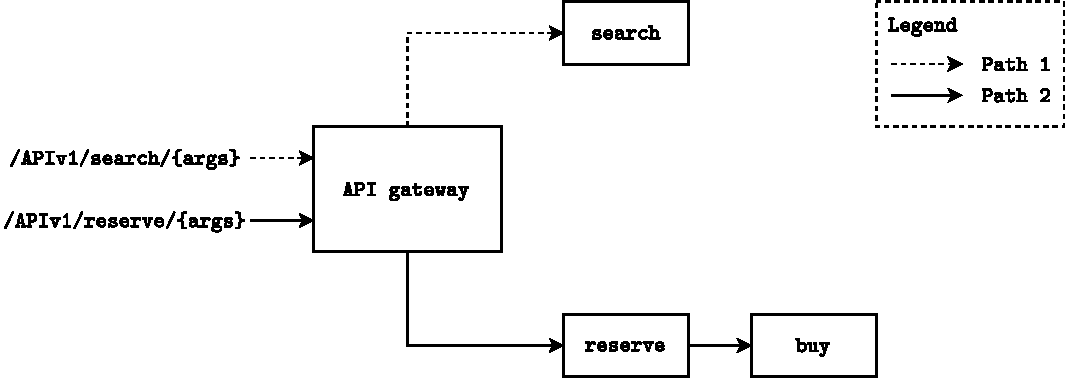
\includegraphics[width=\textwidth]{img/train-ticket-system-1.pdf}
    \caption{Train ticket system.}
    \label{fig: train ticket system}
\end{figure}

\noindent
Microservices run in units deployed onto 2 different Virtual Machines (VMs), \texttt{VM1} and \texttt{VM2} as shown in the following UML deployment diagram.

The available VMs have Computational Resources (CRs) that can be allocated to run microservices. Each VM has a maximum number of CRs and each microservice requires a certain number of CRs, according to the executed artifact. As shown in the schema, available CRs are as follows.
\begin{itemize}
    \item VM1: 20 CRs
    \item VM2: 22 CRs
\end{itemize}
The mapping between microservices and required CRs is as follows.
\begin{itemize}
    \item API gateway: 2 CRs
    \item search: 5 CRs
    \item reserve: 4 CRs
    \item buy: 5 CRs
\end{itemize}
The deployment diagram in Figure~\ref{fig: train ticket deployment diagram} shows that each microservice can be replicated to have redundant business-critical components. In the latter case, requests are directed to all the replicas rather than to an individual instance, and the first answer received from a replica is returned to the caller, while the others are simply ignored. The number of replicas for each microservice shall be defined so that the following nonfunctional requirement is satisfied and the deployment constraints defined in the deployment diagram and above are fulfilled.

\highspace
$R_{1}$: \dquotes{\emph{Both search and reserve services exposed through API gateway shall have availability greater than or equal to 0.99.}}

\begin{figure}[!htp]
    \centering
    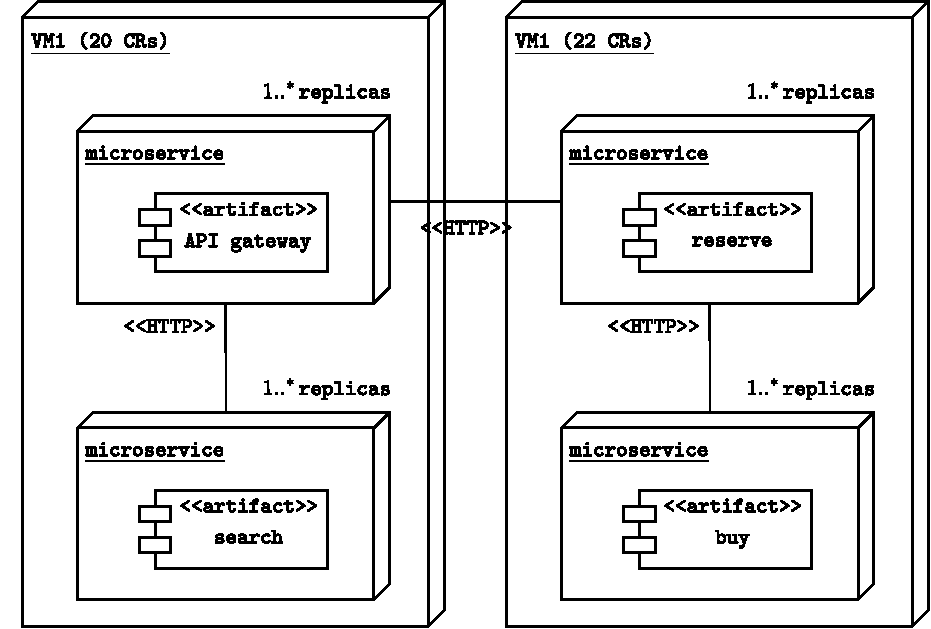
\includegraphics[width=\textwidth]{img/train-ticket-system-2.pdf}
    \caption{Train ticket deployment diagram.}
    \label{fig: train ticket deployment diagram}
\end{figure}

\questionproblem
\begin{enumerate}
    \item Considering the constraints of the execution environment represented, determine whether requirement $R_{1}$ can be satisfied or not assuming the following availability estimates for each microservice.
    \begin{itemize}
        \item API gateway: 0.99
        \item search: 0.98
        \item reserve: 0.95
        \item buy: 0.9
    \end{itemize}

    \item Consider the problem of resource allocation taking into account the operational profile, that is, the behavior of the users. Assume the following workload in terms of average number of concurrent users for each requests.
    \begin{enumerate}
        \item search: 50 users
        \item reserve: 90 users
    \end{enumerate}
    Assume that for reserve, only 20\% of users complete the purchase at reservation time. This means that 20\% of reserve requests get through and reach the buy microservice, while 80\% of them terminate the execution without calling buy. After a preliminary analysis, we realize that availability depends on the workload according to the estimates presented in Table~\ref{table: microservices availability under different workloads}. Does the execution environment have enough computational resources to support the workload defined above still fulfilling requirement $R1$ and the defined constraints? Justify your answer.
    \begin{table}[!htp]
        \centering
        \begin{tabular}{@{} l l | l l @{}}
            \toprule
            \multicolumn{2}{c}{\textbf{LOW workload}} & \multicolumn{2}{c}{\textbf{HIGH workload}} \\
            \multicolumn{2}{c}{0-60 concurrent users} & \multicolumn{2}{c}{60-150 concurrent users} \\
            \cmidrule{1-4}
            \textbf{Microservice} & \textbf{Availability} & \textbf{Microservice} & \textbf{Availability} \\
            \midrule
            \texttt{API gateway} & 0.99 & \texttt{API gateway} & 0.98 \\
            \texttt{search} & 0.98 & \texttt{search} & 0.95 \\
            \texttt{reserve} & 0.95 & \texttt{reserve} & 0.93 \\
            \texttt{buy} & 0.91 & \texttt{buy} & 0.90 \\
            \bottomrule
        \end{tabular}
        \caption{Microservices availability under different workloads.}
        \label{table: microservices availability under different workloads}
    \end{table}
\end{enumerate}

\solution
\textbf{\underline{Solution 1}.} The requirement $R1$ can be satisfied if both virtual machines respect the constraints about the computational resources (CR) and the constraints about the availability percentage. 

To analyze the constraint about the CRs, we need to write two simple inequations:
\begin{equation*}
    \begin{cases}
        2x + 5y \le 20 \\
        4u + 5z \le 22
    \end{cases}
\end{equation*}
Where the first one refers to \texttt{VM1} and the second refers to \texttt{VM2}. To the right side, we have the computational resource limit; to the left, we have a sum of the microservices inside each Virtual Machine. The unknown variables indicate \dquotes{\emph{how many resources are requested}}. For example, if $x$ will be $5$, the API gateway has a request equal to $10$ ($5 \times 2$).

With the same logic, we can write about the inequations in availability. We use the same unknown variables because the computational resources directly affect the availability calculation.
\begin{equation*}
    \begin{cases}
        \left(1-\left(1-0.99\right)^{x}\right) \cdot \left(1-\left(1-0.98\right)^{y}\right) \ge 0.99 \\
        \left(1-\left(1-0.99\right)^{x}\right) \cdot \left(1-\left(1-0.95\right)^{u}\right) \cdot \left(1-\left(1-0.91\right)^{z}\right) \ge 0.99
    \end{cases}
\end{equation*}
To the right side, we have the value accepted by the request $R1$; as a symbol, we use $\ge$ because the request says \dquotes{\emph{[...] availability greater than or equal to 0.99.}}; finally, to the left, we have any component written using the parallelization formula. The reason is that if we have multiple computational resources at a time, we need a duplication. An example of a valid assignment can be:
\begin{equation*}
    x = 2, y = 2, u = 3, z = 2
\end{equation*}

\highspace
\textbf{\underline{Solution 2}.} On time $t$, we have 50 users who request the search microservice and 90 who request the reserve service. Then, the \texttt{API gateway} module will receive 140 ($50 + 90$) concurrent users, and its workload will be \texttt{HIGH} (determined by looking at the Table~\ref{table: microservices availability under different workloads}).

The \texttt{search} module will receive 50 concurrent requests, and looking at the table; its workload will be \texttt{LOW}.

The \texttt{reserve} module must manage 90 concurrent requests, and its workload will be \texttt{HIGH}. 

Finally, the \texttt{buy} module will receive only 18 concurrent requests (20\% of 90 requests), and its workload will be \texttt{LOW}. Then summarizing:
\begin{itemize}
    \item \texttt{API gateway}: 140 users (\texttt{HIGH}) $\rightarrow$ 0.98 availability

    \item \texttt{search}: 50 users (\texttt{LOW}) $\rightarrow$ 0.98 availability

    \item \texttt{reserve}: 90 users (\texttt{HIGH}) $\rightarrow$ 0.93 availability

    \item \texttt{buy}: 18 users (\texttt{LOW}) $\rightarrow$ 0.91 availability
\end{itemize}
The availability inequations written in the previous solution it is modified as follows:
\begin{equation*}
    \begin{cases}
        \left(1-\left(1-0.0.98\right)^{x}\right) \cdot \left(1-\left(1-0.98\right)^{y}\right) \ge 0.99 \\
        \left(1-\left(1-0.0.98\right)^{x}\right) \cdot \left(1-\left(1-0.93\right)^{u}\right) \cdot \left(1-\left(1-0.91\right)^{z}\right) \ge 0.99
    \end{cases}
\end{equation*}
An optimal resource allocation is represented by the assignment:
\begin{equation*}
    x = 2, y = 2, u = 3, z = 2
\end{equation*}
That is again feasible according to environment constraints.